\section{Pianificazione}
La fase di pianificazione consiste nella suddivisione del lavoro tra i vari componenti di \Gruppo. La suddivisione deve essere equa e deve fare in modo che ogni componente abbia la possibilità di ricoprire almeno una volta tutti i ruoli.
\Gruppo ha determinato cinque periodi principali per suddividere il lavoro:
\begin{itemize}
\item analisi;
\item consolidamento dei requisiti;
\item progettazione architetturale;
\item progettazione di dettaglio e codifica;
\item validazione e collaudo.
\end{itemize}
Ognuno di questi periodi viene suddiviso in diverse fasi dove vengono individuate le attività che verranno realizzate.
Infine ogni periodo viene riassunto nel corrispettivo diagrammi di Gantt.
\subsection{Analisi}
Questo periodo ha inizio il 2020-11-09 procede con quattro fasi fino al 2021-01-11.
Durante il decorso di questo periodo i ruoli attivi sono:
\begin{itemize}
\item \textit{responsabile};
\item \textit{amministratore};
\item \textit{analista};
\item \textit{verificatore}.
\end{itemize}
Le precondizioni sono:
\begin{itemize}
	\item formazione del gruppo;
	\item presentazione dei capitolati.
\end{itemize}
Le postcondizioni sono:
\begin{itemize}
	\item scelta del nome e logo del gruppo;
	\item creazione della e-mail;
	\item scelta del capitolato su cui svolgere il progetto;
	\item redazione dei documenti quali: \textit{Studio di fattibilità}, \textit{Norme di Progetto}, \textit{Piano di Progetto}, \textit{Glossario}, \textit{Lettera di Presentazione}, \textit{Piano di Qualifica}, \textit{Analisi dei Requisiti}, ed i verbali;
	\item verifica e approvazione dei documenti.
\end{itemize}
\subsubsection{Attività}
Questo periodo è composto da sette attività che corrispondono ai documenti prodotti:
\begin{itemize}
	\item \textbf{Studio di Fattibilità:} viene fatta una discussione su ogni capitolanto, rilevando i pro e i contro di ognuno di essi, e dopo un periodo di studio e analisi \Gruppo pone la sua preferenza in uno dei capitolati proposti;
	\item \textbf{Norme di Progetto:} vengono definite tutte le regole che \Gruppo dovrà rispettare durante lo sviluppo del progetto, tra cui norme relative al prodotto da realizzare e ai processi da adottare;
	\item \textbf{Individuazione degli strumenti:} consiste nel determinare quali strumenti devono essere utilizzati dal gruppo; vengono ricercati strumenti per la comunicazione, per la stesura dei documenti, per lo sviluppo e la verifica del softwre;
	\item \textbf{Analisi dei Requisiti:} viene analizzato il capitolato scelto nell'attività di Studio di Fattibilità e vengono identificanti i requisiti del capitolato. Il documento viene composto dagli Analisti;
	\item \textbf{Piano di Progetto:} Attività di pianificazione dei compiti e suddivisione dei ruoli. Viene calcolato il preventivo per la realizzazione di progetto. Il documento viene composto dal responsabile;
	\item \textbf{Piano di Qualifica:} si individuano i metodi necessari a garantire la qualità del prodotto. Viene redatto dall'Amministratore e dal Progettista;
	\item\textbf{Glossario:} si individuano tutti i termini che possono risultare ambigui e vengono affiancati da una definizione all'interno del documento;  
	\item \textbf{Lettera di Presentazione:} Documento in cui il gruppo \Gruppo si candida come fornitore del prodotto software richiesto.
\end{itemize}
\subsubsection{Fasi}
la pianificazione di questo periodo è stata suddivisa nelle seguenti sotto-fasi
\begin{itemize}
	\item \textbf{dal 2020-11-09 al 2020-11-30:}
	\begin{itemize}
	\item vengono prese decisioni riguardanti: il nome del team, l'indirizzo e-mail, il logo, la frequenza degli incontri, gli strumenti per la comunicazione;
	\item viene svolta la discussione sui capitolati, eponendo le preferenze personali dei membri del gruppo. Viene dunque analizzato ogni capitolato, ponendo attenzione ai pro e contro di ogni capitolanto e viene fatta una breve valutazione rischi per ognuno. Successivamente si puo dunque inizare la stesura dello Stusio di Fattibilità;
	\item vengono stesi i verbali interni relativi alle riunioni del gruppo durante questa sotto-fase.
	\end{itemize}
	\item \textbf{dal 2020-12-01 al 2020-12-21:}
	\begin{itemize}
		\item viene iniziata la stesura delle \textit{Norme di Progetto} per fissare le regole delle attività del gruppo;
		\item inizio della stesura del \textit{Piano di Progetto}, dove viene descritta la pianificazione del lavoro da svolgere e la suddivisione dei ruoli tra i membri del gruppo;
		\item inizio stesura del \textit{Glossario}, registrando i termini usati nei documenti che risultano ambigui;
		\item stesi i verbali interni relativi agli incontri svoltesi durante questa sotto-fase.
	\end{itemize}
	\item \textbf{dal 2020-12-22 al 2021-01-07:}
	\begin{itemize}
		\item il gruppo inizia ad analizzare il capitolato scelto, ricercando i requisiti e procedendo con la stesura dell'\textit{Analisi dei Requisiti};
		\item Si procede con la stesura del \textit{Piano di Qualifica}, individuando i metodi per garantire la qualità del prodotto;
		\item stesura della \textit{Lettera di Presentazione};
		\item Stesi i verbali interni relativi agli incontri svoltesi durante questa sotto-fase.
	\end{itemize}
	\item \textbf{dal 2021-01-08 al 2021-01-11 :}
	\begin{itemize}
		\item viene completata la stesura del \textit{Glossario};
		\item il gruppo uniforma tutti i documenti prodotti alle regole stabilite nelle \textit{Norme di Progetto} se necessario;
		\item vengono svolte le ultime attività di verifica sui documenti.
	\end{itemize}
\end{itemize}

\subsubsection{Diagramma di Gantt: analisi}
\begin{figure}[H]
    \centering
    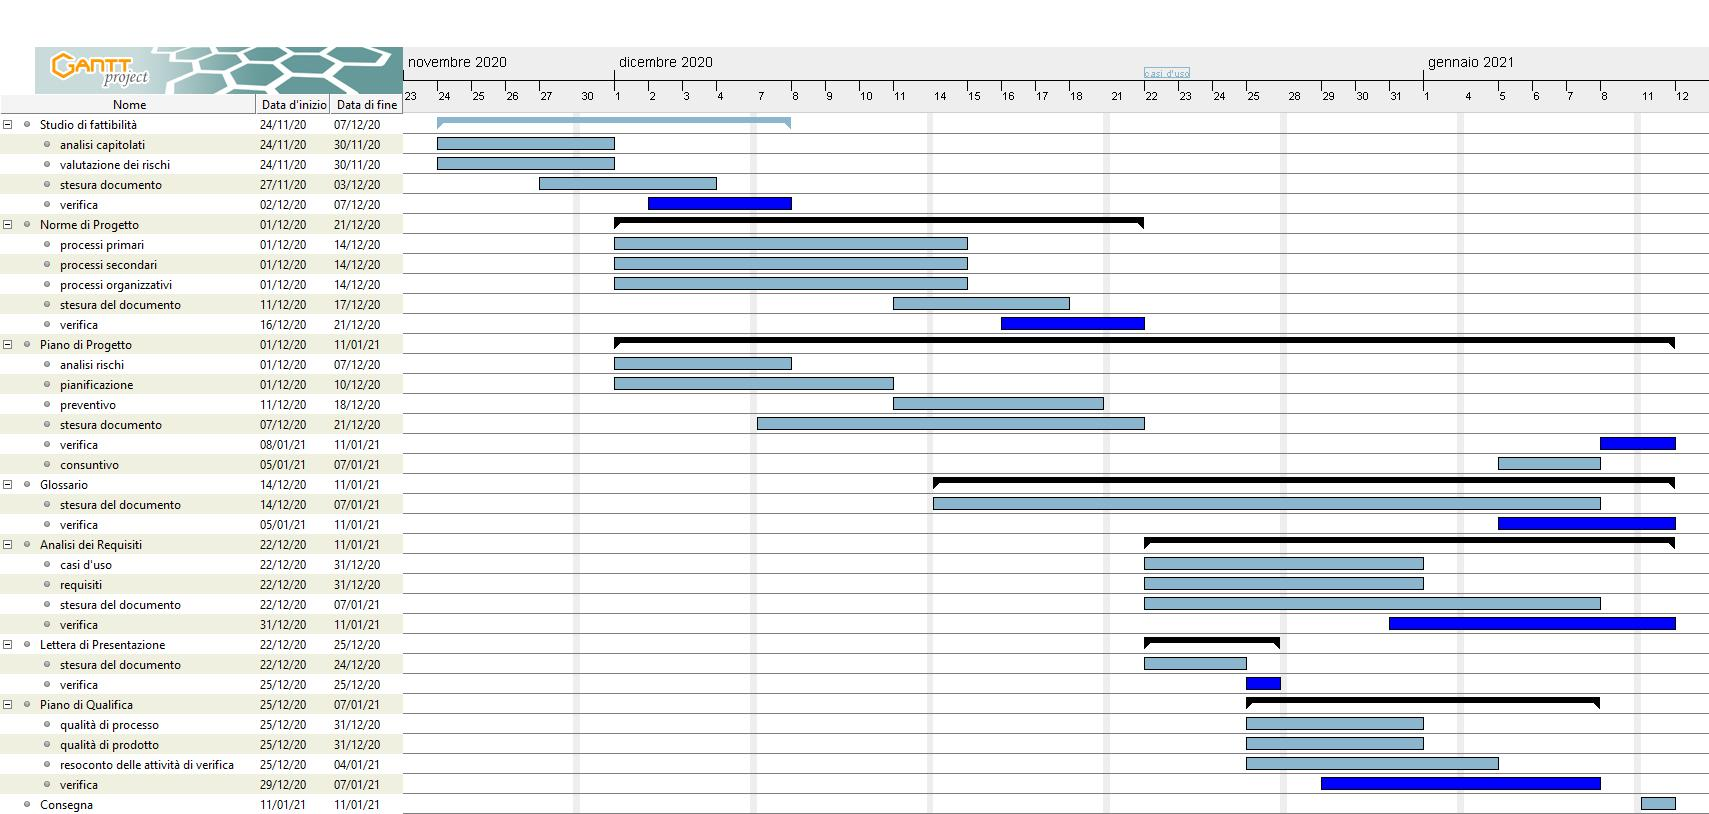
\includegraphics[scale = 0.25]{components/img/Analisi.jpg}
    \caption{Diagramma di Gantt della fase di Analisi}
    \label{fig:Diagramma di Gantt, fase di Analisi}
\end{figure}

\newpage
\subsection{Consolidamento dei Requisiti}
Questo periodo ha una durata dal 2021-01-12 al 2021-01-18.
le precondizioni sono:
\begin{itemize}
	\item le postcondizioni della fase precedente;
	\item consegna dei documenti richiesti.
\end{itemize}
Le postcondizioni sono:
\begin{itemize}
	\item conclusa la preparazione della presentazione da esporre per la Revisione dei Requisiti;
	\item i componenti devono essere preparati per l'utilizzo delle tecnologie necessarie.
\end{itemize}
\subsubsection{Attività}
Le attività che vengono svolte sono:
\begin{itemize}
	\item miglioramento dei documenti e verifica;
	\item preparazione alla presentazione per la Revisione dei Requisiti;
	\item studio autonomo che ogni componente dovrà dedicare per approfondire le tecnologie necessiarie nelle prossime fasi.
\end{itemize}
\subsubsection{Diagramma di Gantt: Consolidamento dei Requisiti}
\begin{figure}[H]
    \centering
    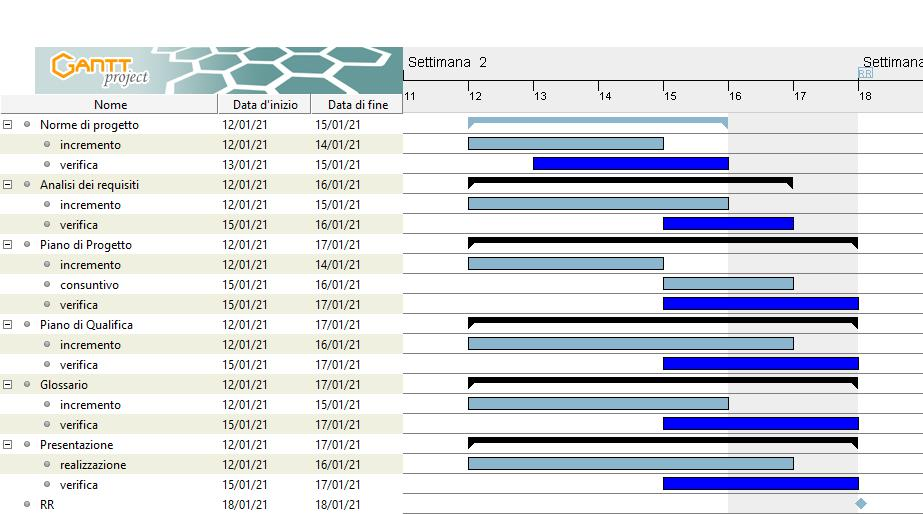
\includegraphics[scale = 0.4]{components/img/consolidamento_requisiti.jpg}
    \caption{Diagramma di Gantt della fase di Consolidamento dei Requisiti}
    \label{fig:Diagramma di Gantt, fase di Consolidamento dei Requisiti}
\end{figure}

\newpage
\subsection{Progettazione architetturale}
Questo periodo ha inizio il 2021-01-19 e si conclude il 2021-03-08.
Le precondizioni sono:
\begin{itemize}
	\item le postcondizioni del periodo precedente;
	\item è stata approvata la candidatura del gruppo al progetto \NomeProgetto.
\end{itemize}
Le postcondizioni sono:
\begin{itemize}
	\item correzione ed incremento dei documenti documenti già prodotti;
	\item produzione del \textit{Proof of Concept} e dell'Allegato Tecnico;
	\item completamento della progettazione ad alto livello del software;
	\item consegna dei documenti richiesti alla Revisione di Progettazione; 	
	\item conclusa la preparazione della presentazione da esporre in sede di revisione.
\end{itemize}
\subsubsection{Attività}
Le attività da svolgere durante il periodo sono:
\begin{itemize}
	\item \textbf{Incremento e Verifica:} i documenti già prodotti vengono migliorati e aggiornati se necessario (\textit{Norme di Progetto}, \textit{Piano di Progetto}, \textit{Glossario},\textit{Piano di Qualifica}, \textit{Analisi dei Requisiti});
	\item \textbf{Technology Baseline:} viene fatta un'analisi ad alto livello del software e viene redatto l'Allegato Tecnico dove vengono individuati i design pattern che verranno addottati per lo sviluppo. Infine viene codificato il \textit{Proof of Concept}, il quale viene presentato o condiviso al committente e proponente in una data da definirsi.
\end{itemize}
\subsubsection{Diagramma di Gantt: progettazione architetturale}
\begin{figure}[H]
    \centering
    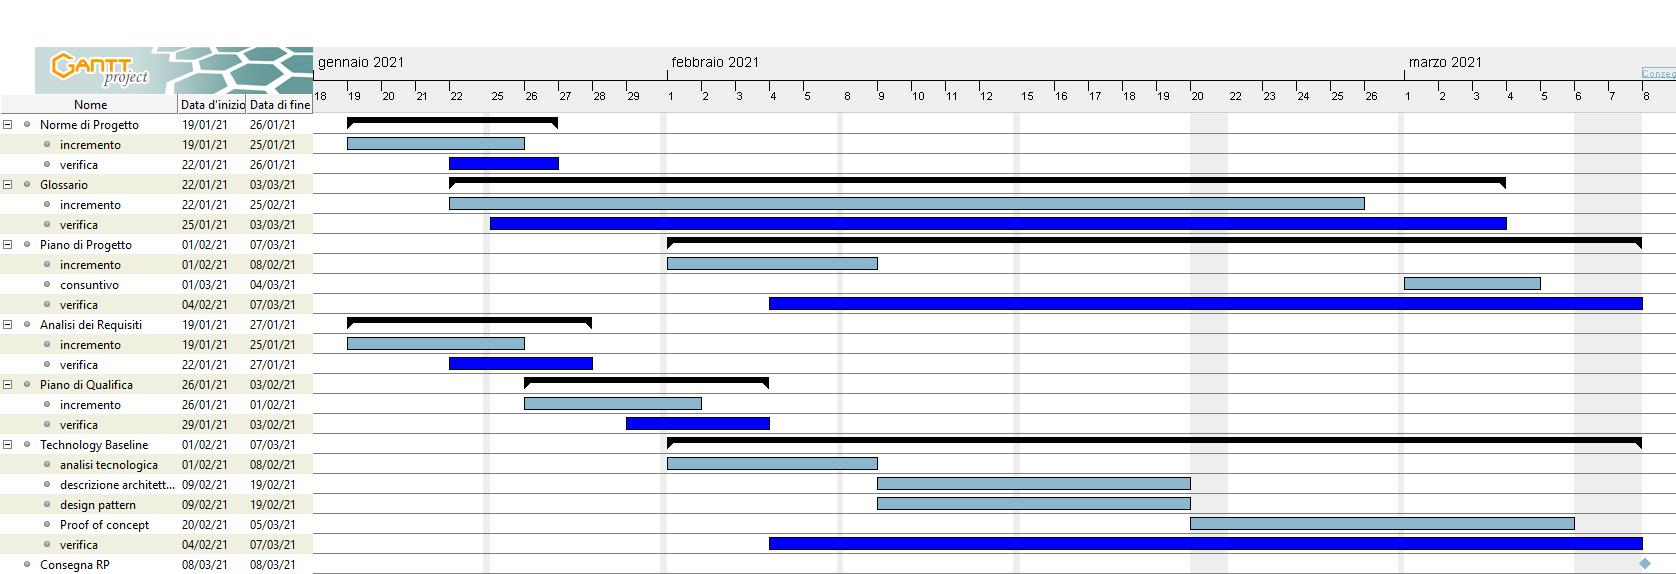
\includegraphics[scale = 0.25]{components/img/progettazione_architetturale.jpg}
    \caption{Diagramma di Gantt della fase di Progettazione Architetturale}
    \label{fig:Diagramma di Gantt, fase di Progettazione Architetturale}
\end{figure}

\newpage
\subsection{Progettazione di dettaglio e codifica}
Questo periodo ha inizio il 2021-03-09 e si conclude il 2021-04-09.
Le precondizioni sono:
\begin{itemize}
	\item aggiornamento e correzione dei documenti;
	\item definizione dell'architettura ad alto livello per il software;
	\item  superamento del colloquio per la \textit{Technology Baseline}.
\end{itemize}
Le postcondizioni sono:
\begin{itemize}
	\item aggiornamento e correzione dei documenti;
	\item stesura del \textit{Manuale Utente};
	\item stesura della \textit{Specifica Tecnica};
	\item superamento del colloquio per la \textit{Product Beseline};
	\item completamento della codifica e la relativa verifica del prodotto software.
\end{itemize}
\subsubsection{Attività}
Le attività che vengono svolte sono:
\begin{itemize}
	\item \textbf{Incremento e verifica:} vengono aggiornati e migliorati i documenti(\textit{Norme di Progetto}, \textit{Piano di Progetto}, \textit{Glossario},\textit{Piano di Qualifica}, \textit{Analisi dei Requisiti}, \textit{Technology Baseline});
	\item \textbf{Product Baseline:} segue la \textit{Technology Baseline}, vengono analizate più in dettaglio le unità i design pattern, le classi e le attività necessarie alla codifica;
	\item \textbf{Specifica Tecnica:} documento contenente tutte le caratteristiche del prodotto e le motivazioni che hanno portato alla loro scelta;
	\item \textbf{Codifica:} questa attività consiste nella scrittura del codice e della sua verifica;
	\item \textbf{Manuale Utente:} viene redatto un documento che descrive tutte le istruzioni d'uso per l'utente.
\end{itemize}
\subsubsection{Diagramma di Gantt: progettazione di dettaglio e codifica}
\begin{figure}[H]
    \centering
    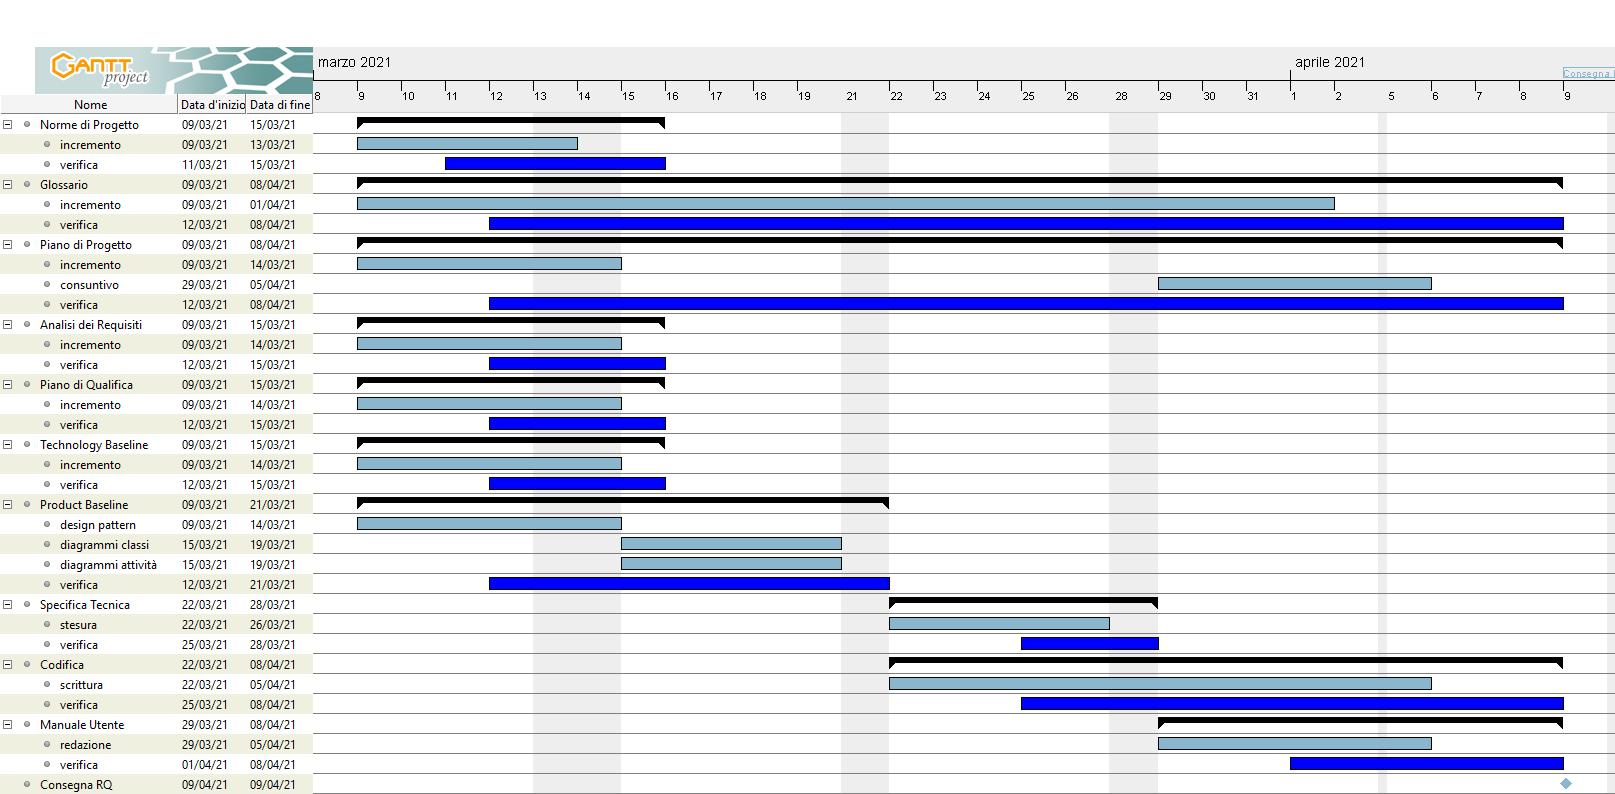
\includegraphics[scale = 0.25]{components/img/progettazione_dettaglio_codifica.jpg}
    \caption{Diagramma di Gantt della fase di Progettazione di Dettaglio e Codifica}
    \label{fig:Diagramma di Gantt, fase di Progettazione di dettaglio e codifica}
\end{figure}

\newpage
\subsection{Validazione e collaudo}
Questo periodo ha inizio il 2021-04-10 e si conclude il 2021-05-10.
Le precondizioni sono:
\begin{itemize}
	\item superamento del colloquio per la Product Baseline;
	\item aggiornamento e correzione dei documenti;
	\item raggiungimento di un prodotto completo, funzionante e di qualità.
\end{itemize}
Le postcondizioni sono:
\begin{itemize}
	\item aggiornamento e correzione dei documenti;
	\item stesura del \textit{Manuale Sviluppatore};
	\item esecuzione dei test di sistema e di accettazione;
	\item consegna dei documenti richiesti alla Revisione di Accettazione.
\end{itemize}
\subsubsection{Attività}
Le attività che vengono svolte sono:
\begin{itemize}
	\item \textbf{Incremento e verifica:} vengono migliorati e aggiornati i documenti già prodotti (\textit{Norme di Progetto}, \textit{Piano di Progetto}, \textit{Glossario},\textit{Piano di Qualifica}, \textit{Analisi dei Requisiti}, \textit{Technology Baseline}, \textit{Product Baseline}, \textit{Specifica Tecnica},\textit{Manuale Utente});
	\item \textbf{Validazione e collaudo:} si eseguiranno ulteriori test sul prodotto, in modo da garantire la correttezza e un buon livello di qualità;
	\item \textbf{Manuale Sviluppatore:} viene redatto il \textit{Manuale Sviluppatore} atto a fornire tutte le informazione necessarie al mantenimento, manutenzione e ampliamento del prodotto.
\end{itemize}
\subsubsection{Diagramma di Gantt: validazione e collaudo}
\begin{figure}[H]
    \centering
    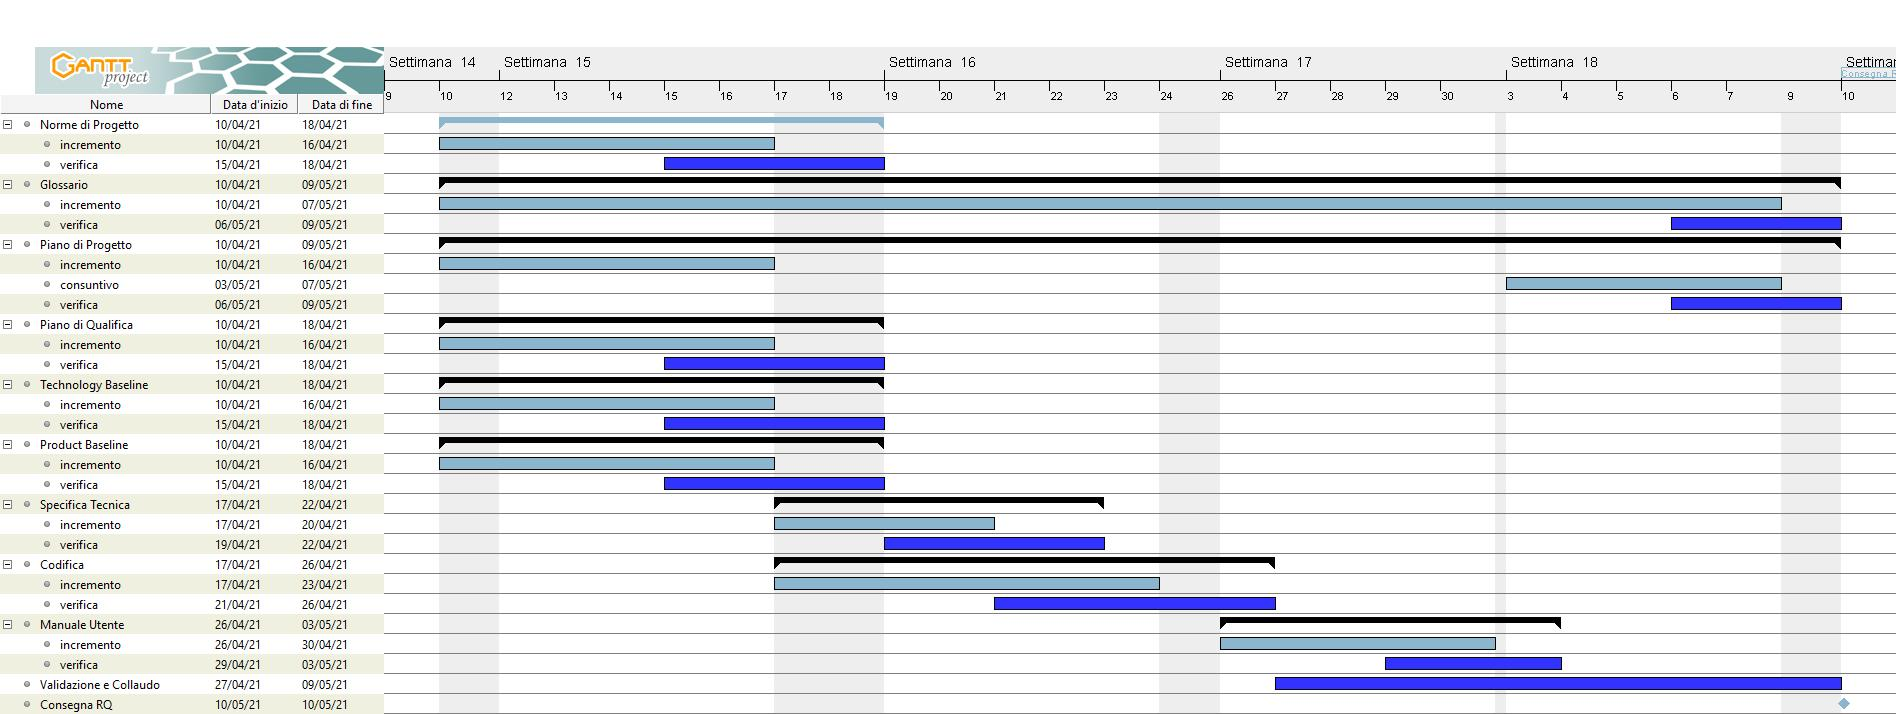
\includegraphics[scale = 0.25]{components/img/validazione_collaudo.jpg}
    \caption{Diagramma di Gantt della fase di Progettazione di Validazione e Collaudo}
    \label{fig:Diagramma di Gantt, fase di Validazione e collaudo}
\end{figure}
